% Setup - do not change
\documentclass[11pt]{article}
\usepackage[top=0.9in, left=0.9in, bottom=0.9in, right=0.9in]{geometry} 
\usepackage{parskip}

\usepackage[english]{babel}
\usepackage[utf8]{inputenc}
\usepackage{amsmath,amsthm,amssymb,graphicx,pdfpages,lipsum,hyperref}
\usepackage[none]{hyphenat}
\usepackage{csquotes}
\usepackage{array}
\usepackage{subcaption}

\setlength\parindent{0pt}

\usepackage[sorting = none]{biblatex}
\addbibresource{references.bib}



\title{\textbf{Optimising NYC Taxi Pick-Up Zones} \\  Predicting Well-Tipped Areas}
\author{
Ngoc Minh Pham \\
Student ID: 1312628 \\
\href{https://github.com/MAST30034-AppliedDataScience/project-1-individual-pnminh-unimelb}{GitHub repo with commit}
}

\begin{document}
\maketitle

\section{Introduction}

Tipping can easily fail to adequately compensate for the effort required, especially for taxi drivers, in cases where the trip involves navigating heavy traffic or extreme weather, handling luggage, or dealing with unpleasant passengers. This imbalance can leave drivers underpaid and undervalued for the full scope of their work. Given that the market is now being dominated by ride-hailing services \cite{ride_hailing_domination}, taxi drivers need to find a way to increase their compensation besides the meagre salary \cite{taxi_driver_salary}.

In this report, we will predict the best areas for traditional yellow taxi drivers to pick up passengers with respect to average tip amount per mile, which is the primary scale of comparison between areas.

\section{Datasets}

The main dataset for this analysis will be from \textbf{TLC Trip Record Data} that includes all records for yellow taxi trip records from the time period of 1/2023 to 12/2023.

An additional dataset being used is the NYC Central Park weather dataset from \textbf{National Centers for Environmental Information}, which provides multiple weather features in NYC, reported hourly and will support the analysis \cite{weather_data}. We assume for trips that involve unfavourable weather conditions, the tip amount will increase since the effort given will be more intensive for drivers. 

\section{Preprocessing}

\subsection{Trip records data}

\subsubsection{Data wrangling}

Inspecting the dataset, we can notice there are several problems that make the records (trips) become invalid. We will handle these issues and see how much data was preserved after the filtering process\cite{sample_solution}.

\begin{itemize}
    \item A new feature \textit{trip duration minutes} will be added to filter records that have negative duration, and will also be capped at 5 hours (300 minutes).
    \item Two new features, \textit{pickup date} and \textit{dropoff date}, will be added to filter records that are not entirely in our analysing period.
    \item Records with negative values for monetary features such as \textit{extra}, fares, surcharges, … were filtered. Additionally, \textit{fare amount} and \textit{total amount} needs to be at lease 2.5 USD, the initial trip fee stated by the TLC.
    \item Records will be considered reasonable trips as they travel at least 0.5 mile (0.8 km) and longer than a minute, given that they may have to pay more in taxes and surcharges than the actual fare amount.
    \item Outliers will be handled by choosing the 99.99 percentile of the feature, since using the IQR method would remove too much data.
\end{itemize}

\subsubsection{Feature engineering and Feature selection}

For the analysis question, we will group \textit{pickup location ID} and \textit{dropoff location ID} to boroughs, according to \textbf{taxi zones data} provided by the TLC website.

\begin{itemize}
    \item Preprocessed data from previous procedure will be mapped into 6 boroughs based on pick up and drop off location. 
    \item Mapped records that have either \textit{pickup zone} or \textit{dropoff zone} outside NYC boroughs will be filtered, since those data may not be useful for our analysis.
    \item Original datetime features, (\textit{pickup datetime}, \textit{dropoff datetime}), are dropped since the modelling process will not involve with such unique features.
    \item Selecting only records with \textit{payment type} as card payments, since cash tips are not recorded, according to the data provider. The \textit{payment type} feature is then dropped, since every record has the same value for this feature.
\end{itemize}

\subsection{Weather data}

Observing the weather dataset, despite having a large amount of attributes (91), we can see that most of the attributes have multiple missing entries and using all of them not only may damage the integrity of the original dataset, but also can overfit the data on the weather attributes, and reduce the model performance. After selection\cite{sample_solution}, remaining attributes are:

\begin{itemize}
    \item date
    \item hour
    \item tmp (temperature)
    \item dew (dew point)
    \item atm (atmosphere pressure)
\end{itemize}

\subsection{Final dataset}

The final dataset is the merge between the processed trip records dataset and the processed weather dataset, and will be used for further visualising, modelling and analysing.

\section{Visualisation and Prior Analysis}

Before proceeding to train and predict the datasets with our models, we want to have a look at the distribution of the data to see if our analysis can support the distribution, or can reveal any underlying trend that can not be seen easily.

\begin{figure}[h]
    \includegraphics[width=0.5\textwidth]{plots/geospatial.png}
    \centering
    \caption{Distribution of average tip amount per mile in NYC}
\end{figure}

As shown in the visualisation (Figure 1), the top 10 pickup locations with the highest average tip amount per mile are mostly in the Manhattan borough. The original values for the data distribution consist of an outlier for a location in Staten Island, so we applied square root transformation (monotonic function for non-negative values) for the data, which can mitigate the effect in our visualisation.

While there are some locations outside this borough also have a noticeable value, this next plot will support the distribution that Manhattan is the borough with the highest average tip amount over trip distance.

\begin{figure}[h]
    \centering
    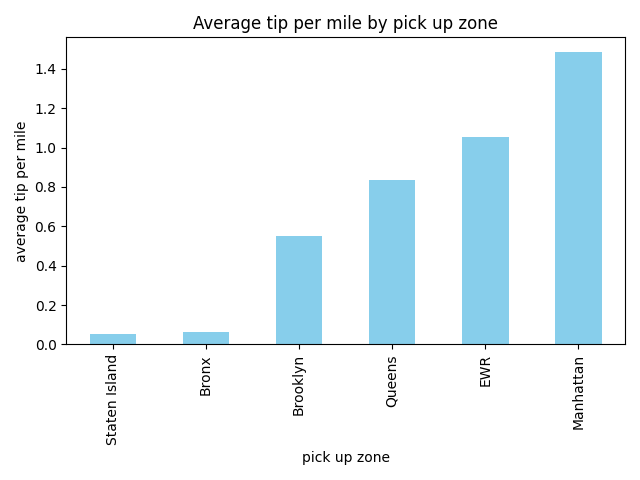
\includegraphics[width=0.5\linewidth]{plots/avg_tip_per_mile_by_zones.png}
    \caption{Average tip amount per mile by pick up boroughs}
\end{figure}

Based on these visualisations (Figure 1 \& 2), it is plausible to assume that the data is distributed differently for each borough, and the next step in the process will require splitting data into boroughs for better performance.

\section{Modelling}

\subsection{Choosing models}

For such a regression task, the most common model would be Linear Regression. We choose this model since it is easy to implement and interpret, and robust to overfitting with regularisation applied. To compare with this model, we choose Random Forest Regression since this model is more robust and flexible for a dataset that does not ensure linear relationships. The records in 12/2023 will be used as the test dataset to evaluate our models trained by data until 11/2023.

\subsection{Selecting features for modelling}

For the sake of fair comparison between mentioned models, we will choose the same feature set for both models prior to training, which may not be the best choice but can reduce the implementation effort and keep the comparison process unbiased for both.

\begin{figure}[h]
    \centering
    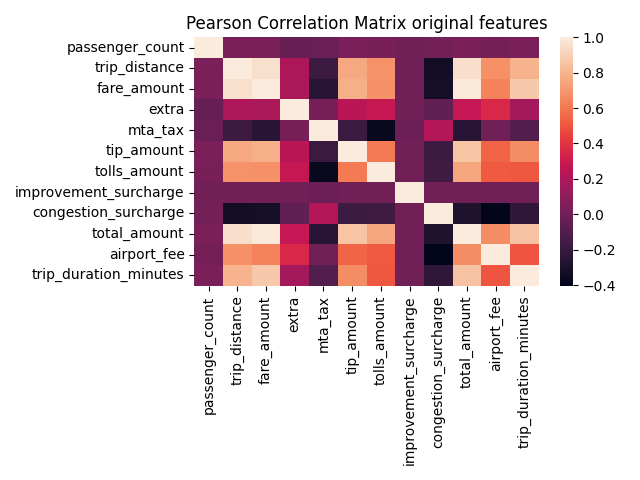
\includegraphics[width=0.65\linewidth]{plots/pearson_correlation_matrix.png}
    \caption{Pearson Correlation Matrix for original numerical features}
\end{figure}

We implemented a simple Pearson correlation matrix between the numerical features of the trip records dataset, leaving out the weather dataset, since including those features can misinterpret the relationships between original features. As shown in the figure, the attributes that have high correlation with our desired label, \textit{tip amount}, are (\textit{trip distance}, \textit{fare amount}, \textit{tolls amount}, \textit{total amount}, \textit{airport fee} and \textit{trip duration}) and were selected for training (Figure 3).

For the weather features, another Pearson correlation matrix is computed to observe the relationships between these additional features and \textit{tip amount}. Surprisingly, contradicting with our assumption, these attributes do not have high correlation with the label (Figure 4), and may not be useful for the modelling process. However, we will proceed with these features to see if this contradiction is accurate.

\begin{figure}[h]
    \centering
    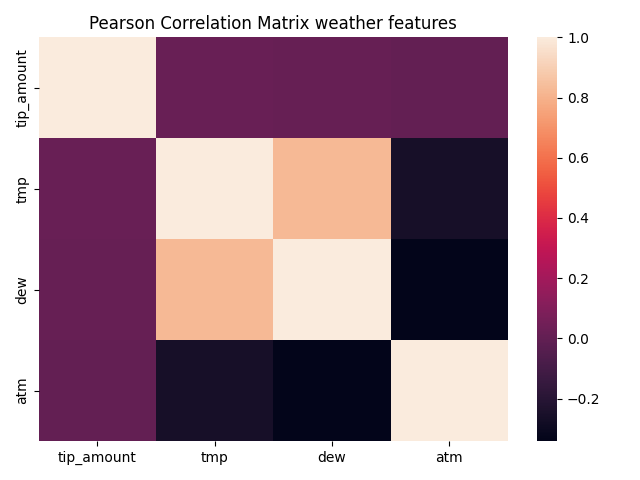
\includegraphics[width=0.5\linewidth]{plots/pearson_correlation_weather_matrix.png}
    \caption{Pearson Correlation Matrix for weather features}
\end{figure}

With categorical features, \textit{store and fwd flag} and \textit{VendorID} will not be used since these attributes have no attribution to the fare and \textit{RatecodeID} will also be dropped since the \textit{fare amount} and \textit{trip distance} can already reveal the rate for the trip. Finally, the datasets will be split into corresponding boroughs, as stated in the prior analysis.

\subsection{Linear Regression}

Since the data is split into boroughs and there is no categorical attributes remaining, we have the following model

\begin{equation}
    Y = X\beta + \epsilon
\end{equation}

where $\beta$ consists of coefficients for attributes set include \textit{trip distance}, \textit{fare amount}, \textit{tolls amount}, \textit{total amount}, \textit{airport fee}, \textit{trip duration}, \textit{tmp}, \textit{dew} and \textit{atm}. 

After the training process with LASSO applied for regularisation, this is the estimate for the coefficients of $\beta$

\begin{table} [h!]
\begin{center}
\begin{tabular}{|m{2.5cm}||m{2cm}|m{1.5cm}|m{1.5cm}|m{1.5cm}|m{2cm}|m{2.5cm}|}
\hline
Attributes & Manhattan & Queens & EWR & Bronx & Brooklyn & Staten Island \\
\hline
\textit{trip distance} & 0 & 0 & -0.047 & 0.054 & -0.052 & 0.042 \\
\textit{fare amount}   & 0 & -0.491 & -0.855 & -0.306 & -0.544 & -0.674 \\
\textit{tolls amount}  & 0 & -0.687 & -0.822 & -0.351 & -0.586 & -0.724 \\
\textit{total amount}  & 0.149 & 0.599 & 0.876 & 0.358 & 0.605 & 0.714 \\
\textit{airport fee}   & 0 & -0.969 & 0 & 0 & 0 & 0 \\
\textit{trip duration} & 0 & -0.005 & -0.002 & -0.012 & -0.018 & -0.007 \\
\textit{tmp} & 0 & 0 & -0.002 & 0 & 0 & 0 \\
\textit{dew} & 0 & 0 & 0 & 0 & 0 & 0 \\
\textit{atm} & 0 & 0 & 0 & 0 & 0 & 0 \\
\hline
\end{tabular}
\caption{Coefficients for Linear Regression models across different boroughs}
\end{center}
\end{table}

The regularised coefficients showed that the weather features did not attribute to the model, opposing to our assumption and validating the prior statement about them. In other words, weather conditions may not affect the tip amount by customers, suggesting that original features play a more substantial role in determining tip amounts. Additionally, \textit{airport fee} is only significant in Queens borough, the borough contains 2 airports JFK and LGA, which suggests that tipping amount in this borough is strongly affected by whether the trip includes airports in its route. Finally, coefficients in the Manhattan borough are all 0 except \textit{total amount}, indicating a consistent tipping behaviour of 15\% of the trip fare, excluding other factors. 

\subsection{Random Forest Regression}

Random Forest Regression is an ensemble of multiple decision trees and therefore, the interpretability is the model attributes is unavailable. However, we can see how important the attributes are by \textit{feature importance} of the model.

\begin{table} [h!]
\begin{center}
\begin{tabular}{|m{2.5cm}||m{2cm}|m{1.5cm}|m{1.5cm}|m{1.5cm}|m{2cm}|m{2.5cm}|}
\hline
Attributes & Manhattan & Queens & EWR & Bronx & Brooklyn & Staten Island \\
\hline
\textit{trip distance} & 0.213 & 0.149 & 0.15 & 0.08 & 0.078 & 0.046 \\
\textit{fare amount}   & 0.259 & 0.183 & 0.181 & 0.2 & 0.243 & 0.39 \\
\textit{tolls amount}  & 0.059 & 0.036 & 0.076 & 0.078 & 0.036 & 0.053 \\
\textit{total amount}  & 0.382 & 0.561 & 0.319 & 0.499 & 0.491 & 0.336 \\
\textit{airport fee}   & 0 & 0.014 & 0 & 0.005 & 0.002 & 0 \\
\textit{trip duration} & 0.087 & 0.057 & 0.149 & 0.087 & 0.148 & 0.09 \\
\textit{tmp} & 0 & 0 & 0.035 & 0.026 & 0.001 & 0.027 \\
\textit{dew} & 0 & 0 & 0.052 & 0.013 & 0.001 & 0.027 \\
\textit{atm} & 0 & 0 & 0.038 & 0.012 & 0.001 & 0.031 \\
\hline
\end{tabular}
\caption{Importance of attributes for Random Forest Regression models across different boroughs}
\end{center}
\end{table}

The importance table indicates that the weather features, despite the small proportion, are having higher attributes to this model compared to Linear Regression, which affect the \textit{tip amount} decided by customers. For Manhattan, there are more features attributing to the model and not only \textit{total amount} like Linear Regression. Additionally, \textit{airport fee} is also only relatively useful in Queens borough.

\section{Model comparison and Discussion}

After training the models, we proceed to predict the \textit{tip amount} for the trip records in the test dataset. The Root Mean Squared Error (RMSE) will be the primary scale, with the support of R² score.

\begin{table}[h!]
\centering
\begin{tabular}{|p{3cm}|p{2cm}|p{2.5cm}|p{2cm}|p{2cm}|}
\hline
Borough & LR RMSE & RFR RMSE & LR R² & RFR R²\\
\hline
Manhattan     & \textbf{1.62}  & 1.662 & \textbf{0.687} & 0.67\\
Queens        & \textbf{2.278} & 3.59  & \textbf{0.846} & 0.617\\
EWR           & \textbf{2.024} & 7.453 & \textbf{0.953} & 0.367\\
Bronx         & \textbf{1.119} & 1.345 & \textbf{0.587} & 0.404\\
Brooklyn      & \textbf{1.239} & 2.694 & \textbf{0.906} & 0.557\\
Staten Island & \textbf{2.458} & 4.087 & \textbf{0.894} & 0.708 \\
\hline
\end{tabular}
\caption{RMSE and R² scores for 6 boroughs.}
\label{tab:scores}
\end{table}

Across the pickup zones, we can see that the RMSE from the Linear Regression model is smaller than that of the Random Forest Regression model, indicating better predictions by the former model. For R², the score for the Linear model is higher for all boroughs, suggesting this model explains a larger proportion of the variance in the data compared to the Random Forest model. 

For specific, EWR borough observe a large difference in both RMSE and R² between the two models, indicating a significant superior model. Additionally, for Bronx borough, while RMSE for both models are the lowest comparing to other boroughs, the R² score is also really low which shows that while the models are good at predicting the \textit{tip amount}, the variance of the data is not properly explained.

After the prediction process, we total the actual \textit{tip amount} and that predicted by the models across boroughs, then divide by the total distance travelled to get the average \textit{tip amount per mile}.

\begin{figure}[h]
    \centering
    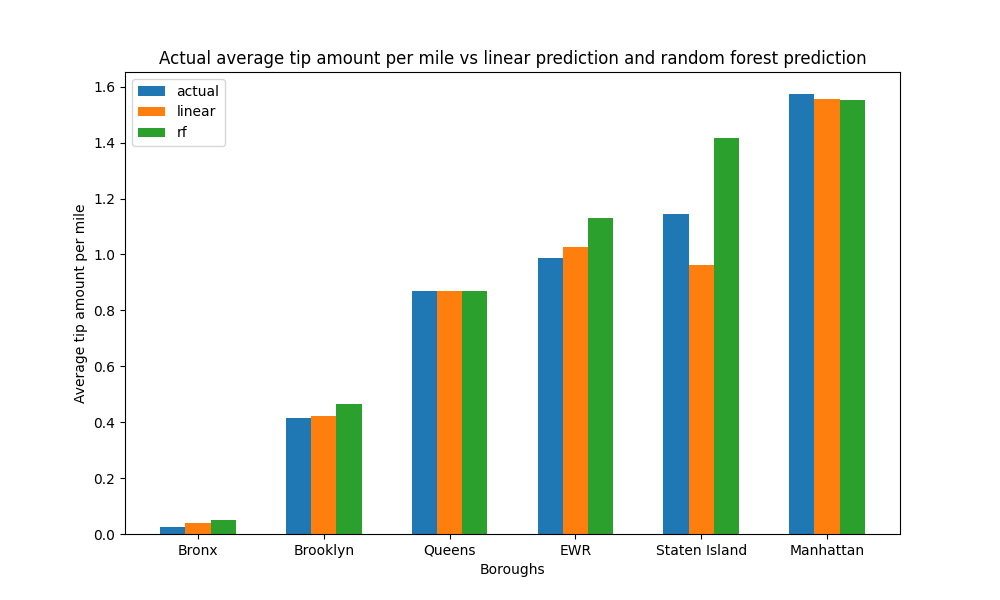
\includegraphics[width=0.7\linewidth]{plots/bar_chart_tip_per_mile_amount.png}
    \caption{Average tip amount per mile by boroughs}
\end{figure}

For the test dataset, the position of Staten Island has changed drastically from the last place to second place with respect to \textit{tip amount per mile}. Moreover, the predictions of both models are quite similar about this behaviour. When we take a closer look, there are only 6 records for Staten Island in the test dataset, and the average \textit{tip amount per mile} value can be affected by outliers (unusual tipping behaviour). Such a small dataset is also unrepresentative, leading to an inaccurate estimate. Finally, despite the problem with Staten Island, both models seem to properly order the boroughs, similar to the actual distribution of the data.

\section{Recommendations}

For further research into this question, we suggest a deeper analysis of external factor other than weather, which did not seems to have any effect, to see how \textit{tip amount} is influenced. For example, tourists who may not familiar with the US tip culture will not be giving tips, or customers on holidays will be more likely to give a more generous tip. However, those examples are only some assumptions and more thorough analysis will be needed. Additionally, we can consider splitting the dataset in another way that makes the dataset more representative for State Island area (larger time period, 80-20 split, …) so that the predictions will not be affected by outliers. Random Forest Regression, in our analysis, seems to be outperformed by Linear Regression, which is not an expected result. This can suggest additional steps in the modelling process such as Hyperparameter tuning or k-fold Cross Validation for further comparsions.

For our target audiences, taxi drivers, the borough to pick up customers will be Manhattan with respect to \textit{tip amount per mile}, which is predicted to be the best place by Linear Regression and second-best place with a small margin by Random Forest Regression (Figure 5). With that being said, drivers should start their routes from locations in the Manhattan borough, and include those locations as their trips' destinations can also improve their total revenue aside prioritising tips without having to travel back to those areas, especially when ratio of live miles (miles with a fare) to cruising miles (miles without a fare) is relatively low for this traditional transportation service \cite{miles_ratio}.

Additionally, if the ratio of tip over effort spent is not the primary concerns, drivers can consider a route including more boroughs other than Manhattan.

\begin{figure}[h]
    \centering
    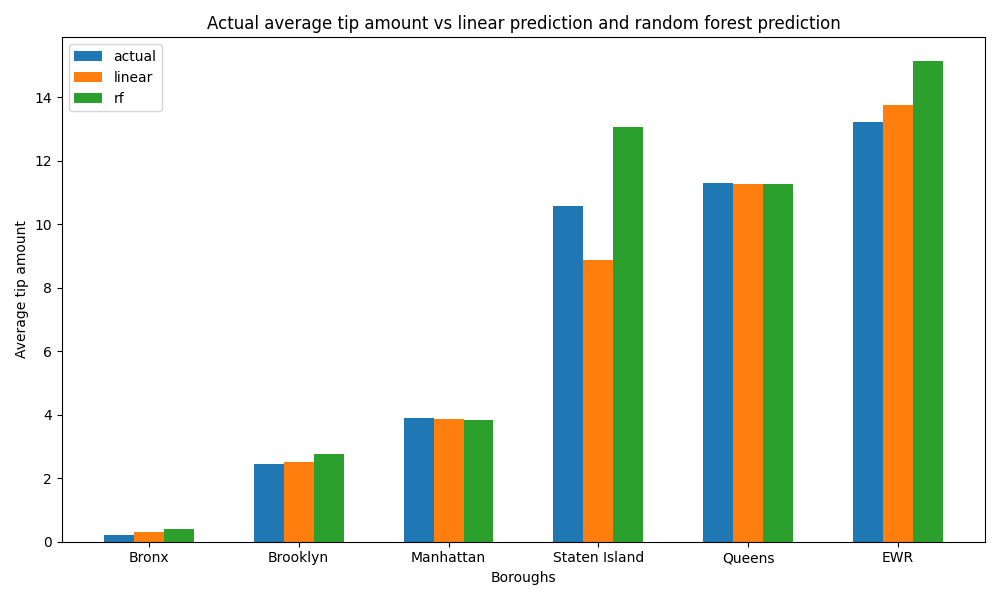
\includegraphics[width=0.7\linewidth]{plots/bar_chart_tip_amount.png}
    \caption{Average tip amount per mile by boroughs}
\end{figure}

Manhattan, despite being the best borough in the \textit{tip amount per mile} scale, is only the fourth-best tipped area out of 6 boroughs (Figure 6), with a noticeable difference. With that modest number, drivers can take into account that other well-tipped areas like Queens or EWR can be a better place to prioritise since the tip pay would be higher than that from Manhattan. After all, drivers can work around these 3 primary areas since they can either get tipped well or get tipped sufficiently for their effort. Staten Island, the unrepresentative borough and the two remaining, Bronx and Brooklyn, should be considered adequately before adding to the route.

\section{Conclusion}

This study aimed to identify the best areas for NYC yellow taxi drivers to optimise their tip earnings by focusing on \textit{tip amounts per mile}. Through a combination of data preprocessing, feature engineering, model selection and feature selection, we proceeded modelling with Linear Regression and Random Forest Regression and compared their performances. Findings indicate that Manhattan consistently offers the highest average \textit{tip amounts per mile}, making it the most advantageous borough for drivers to include in their routes. The results strongly suggest that focusing on Manhattan for both pick-ups and drop-offs can maximise a driver's income while minimising unnecessary cruising miles. Taxi drivers can also include areas with pure high \textit{tip amount} like EWR, Queens and Staten Island to their routes if their primary concern is money

Moving forward, despite weather conditions showing minimal impact on tipping behaviour, the results are promising, and future research could explore other external factors, such as customer demographics or time-specific events, to further refine these strategies. The analysis also underwent an inadequate split method for train and test datasets, resulting in a different distribution for the test dataset. However, ultimately, traditional taxi drivers can still get sufficiently paid despite the poor salary\cite{taxi_driver_salary} if they navigate the route carefully.

\clearpage

% BEGIN REFERENCES SECTION
\printbibliography

\end{document}